\documentclass[]{article}
\usepackage{lmodern}
\usepackage{amssymb,amsmath}
\usepackage{ifxetex,ifluatex}
\usepackage{fixltx2e} % provides \textsubscript
\ifnum 0\ifxetex 1\fi\ifluatex 1\fi=0 % if pdftex
  \usepackage[T1]{fontenc}
  \usepackage[utf8]{inputenc}
\else % if luatex or xelatex
  \ifxetex
    \usepackage{mathspec}
  \else
    \usepackage{fontspec}
  \fi
  \defaultfontfeatures{Ligatures=TeX,Scale=MatchLowercase}
\fi
% use upquote if available, for straight quotes in verbatim environments
\IfFileExists{upquote.sty}{\usepackage{upquote}}{}
% use microtype if available
\IfFileExists{microtype.sty}{%
\usepackage{microtype}
\UseMicrotypeSet[protrusion]{basicmath} % disable protrusion for tt fonts
}{}
\usepackage[margin=1in]{geometry}
\usepackage{hyperref}
\hypersetup{unicode=true,
            pdfborder={0 0 0},
            breaklinks=true}
\urlstyle{same}  % don't use monospace font for urls
\usepackage{graphicx,grffile}
\makeatletter
\def\maxwidth{\ifdim\Gin@nat@width>\linewidth\linewidth\else\Gin@nat@width\fi}
\def\maxheight{\ifdim\Gin@nat@height>\textheight\textheight\else\Gin@nat@height\fi}
\makeatother
% Scale images if necessary, so that they will not overflow the page
% margins by default, and it is still possible to overwrite the defaults
% using explicit options in \includegraphics[width, height, ...]{}
\setkeys{Gin}{width=\maxwidth,height=\maxheight,keepaspectratio}
\IfFileExists{parskip.sty}{%
\usepackage{parskip}
}{% else
\setlength{\parindent}{0pt}
\setlength{\parskip}{6pt plus 2pt minus 1pt}
}
\setlength{\emergencystretch}{3em}  % prevent overfull lines
\providecommand{\tightlist}{%
  \setlength{\itemsep}{0pt}\setlength{\parskip}{0pt}}
\setcounter{secnumdepth}{0}
% Redefines (sub)paragraphs to behave more like sections
\ifx\paragraph\undefined\else
\let\oldparagraph\paragraph
\renewcommand{\paragraph}[1]{\oldparagraph{#1}\mbox{}}
\fi
\ifx\subparagraph\undefined\else
\let\oldsubparagraph\subparagraph
\renewcommand{\subparagraph}[1]{\oldsubparagraph{#1}\mbox{}}
\fi

%%% Use protect on footnotes to avoid problems with footnotes in titles
\let\rmarkdownfootnote\footnote%
\def\footnote{\protect\rmarkdownfootnote}

%%% Change title format to be more compact
\usepackage{titling}

% Create subtitle command for use in maketitle
\newcommand{\subtitle}[1]{
  \posttitle{
    \begin{center}\large#1\end{center}
    }
}

\setlength{\droptitle}{-2em}

  \title{\hfill \large{Albert Garcia}\\
\hfill \large{Jacob Gellman}\\
\hfill \large{Casey O'Hara}\\
\hfill \large{Vincent Thivierge}}
    \pretitle{\vspace{\droptitle}\centering\huge}
  \posttitle{\par}
    \author{\hfill Econ 230B}
    \preauthor{\centering\large\emph}
  \postauthor{\par}
      \predate{\centering\large\emph}
  \postdate{\par}
    \date{\hfill 2019-02-12}


\begin{document}
\maketitle

\newcommand{\EE}{\mathbb{E}}
\newcommand{\eps}{\varepsilon}
\newcommand{\LL}{\mathscr{L}}
\newcommand{\dd}{\partial}

\section{Problem set 5}\label{problem-set-5}

\subsection{Exercises lecture 8}\label{exercises-lecture-8}

\subsubsection{8.1 Every morning, 6,000 commuters must travel from East
Potato to West Potato. There are two ways to make the
trip.}\label{every-morning-6000-commuters-must-travel-from-east-potato-to-west-potato.-there-are-two-ways-to-make-the-trip.}

One way is to drive straight across town, through the heart of Middle
Potato. The other way is to take the Beltline Freeway that circles the
Potatoes. The Beltline Freeway is entirely uncongested, but the drive is
roundabout and it takes 45 minutes to get from East Potato to West
Potato by this means. The road through Middle Potato is much shorter and
if it were uncongested it would take only 20 minutes to make the trip.
Given the current size of the road through Middle Potato, if the number
of commuters using the road is \(N_1\), the time it takes to drive from
East Potato to West Potato by this road is \(20 + N_1/100\).

\begin{enumerate}
\def\labelenumi{\alph{enumi})}
\item
  With the road at its current size and with no tolls, how many
  commuters will use the road through Middle Potato? What will be the
  total number of minutes per morning spent by all commuters going from
  East Potato to West Potato?

  \begin{itemize}
  \tightlist
  \item
    Commuters will decide which road to take based on their utility,
    which without additional information, we assume is directly related
    to how long it takes to get to West Potato, or WePo. Equilibrium
    will occur when the marginal commuter's WePo commute time
    (i.e.~disutility) on the Beltway, or BF, is the same as the time it
    takes to drive through Middle Potato, or MoPo.

    \begin{align*}
      U_{i,BF} &= U_{i,MoPo} &\text{(at equilibrium)}\\
      -45 &= -(20 + \frac{x}{100})\\
      \Rightarrow x &= (45 - 20) * 100  = 2500 
    \end{align*}
  \item
    Once 2500 drivers have chosen the MoPo route, the two commute times
    will be equal and commuters will be indifferent between the two
    routes; if any more were to consider this route, then it would take
    longer and therefore they would opt to take the BF route.
  \item
    All drivers will now take 45 minutes to commute to WePo, so
    \(45 * 6000 = 270,000\) total driver-minutes each morning.
  \end{itemize}
\item
  Suppose that a social planner controlled access to the road through
  Middle Potato and chose the number of commuters who were allowed to
  use the Middle Potato road in such a way as to minimize the sum of the
  number of minutes spent by commuters traveling from East Potato to
  West Potato. How many commuters would the social planner permit to use
  the Middle Potato road each morning? How long would it then take the
  commuters who used this road to make their morning commute?

  \begin{itemize}
  \tightlist
  \item
    The social planner will minimize the total commuting time
    (i.e.~maximize utility), dividing commuters into \(x\) taking the
    MoPo route and \((6000 - x)\) taking the BF route:

    \begin{align*}
      U_{tot} = \sum U_i &= \sum_{i-1}^{x} -(20 + \frac{x}{100}) + \sum_{i=x+1}^{6000} -45\\
    &= -20x - \frac{x^2}{100} - 45 (6000 - x)\\
      \frac{\dd U_{tot}}{\dd x} &= 25 - \frac{x}{50} = 0 &\text{(first order cond'ns)}\\
      \Rightarrow x &= 1250
    \end{align*}
  \item
    The commute for drivers taking the BF route will still take 45
    minutes; the commute for drivers assigned to take the MoPo will take
    only \(20 + x/100 = 32.5\) minutes.
  \item
    Total commute time for the entire EPo community is
    \(45 (6000 - x) + 32.5x = 254,375\) minutes.
  \end{itemize}
\item
  Suppose that commuters value time saved from commuting at \(\$w\) per
  minute. Suppose that the government charges a toll for driving on the
  road through Middle Potato and divides the revenue from the toll
  equally among all 6,000 commuters. If the government's objective is to
  minimize the total amount of time that people spend commuting, how
  high should it set the toll? How much revenue will it collect? With
  this policy, how much better off (evaluated in dollars) is each
  commuter than they were in the equilibrium with no tolls?

  \begin{itemize}
  \tightlist
  \item
    The toll should be set such that the marginal commuter is
    indifferent between the BF route and MoPo route at the
    time-minimizing levels, to ensure equilibrium.

    \begin{align*}
      U_{BF}   &= -45w + \frac{tx}{6000} 
    &\text{(time disutility plus rebate)}\\
      U_{MoPo} &= -(20 + \frac{x}{100})w - t + \frac{tx}{6000}
    &\text{(time disutility minus tax plus rebate)}\\
      \Rightarrow -45w + \frac{tx}{6000} &= -20w - \frac{wx}{100} - t + \frac{tx}{6000}\\
      \Rightarrow t &= (25 - \frac{x}{100})w\\
    &= 12.5w &\text{(substitute $x = 1250$)}
    \end{align*}
  \item
    At this level, the tax will generate
    \(tx = 12.5x \times 1250 = \$15,625w\) of revenue.
  \item
    Relative to the no-toll equilibrium, the BF drivers are
    \(+\frac{tx}{6000} = \$2.6w\) better off; because the system is at
    equilibrium, the MoPo drivers are better off by the same amount
    relative to the no-toll equilibrium. We can also consider that the
    utility loss due to the tax on the MoPo drivers exactly cancels the
    utility gain of the reduced commute time; therefore, the net utility
    gain is just the rebate term.
  \end{itemize}
\end{enumerate}

\subsubsection{8.2 Suppose that a monopolist controls the road through
Middle Potato and sets the toll that maximizes total
revenue.}\label{suppose-that-a-monopolist-controls-the-road-through-middle-potato-and-sets-the-toll-that-maximizes-total-revenue.}

What price will the monopolist set and how many people will use the road
at this price? How does this price compare with the optimal toll?

\begin{quote}
\textbf{Hint}: \emph{First find the ``demand curve'' relating number of
users to price. Then find the revenue-maximizing quantity and price.}
\end{quote}

\begin{itemize}
\tightlist
\item
  Demand for access to the MoPo route is based on the price of the toll;
  demand will be at equilibrium when utility for commuter \(i\) are
  equal: \(U_{i,BF} = U_{i,MoPo}\).
\end{itemize}

\begin{align*}
  U_{BF}   &= -45w 
    &\text{(time disutility only)}\\
  U_{MoPo} &= -(20 + \frac{x}{100})w - t
    &\text{(time disutility minus toll)}\\
  \Rightarrow t &= (25 - \frac{x}{100})w &\text{(same as 8.1c)}\\
  \Rightarrow x &= 2500 - 100\frac{t}{w}
\end{align*}

\begin{itemize}
\tightlist
\item
  Total revenue is then \(R = xt = 2500t - \frac{100}{w}t^2\).
\end{itemize}

\begin{align*}
  \frac{\dd R}{\dd t} &= 2500 - \frac{200}{w}t = 0\\
  \Rightarrow t &= 12.5w
\end{align*}

\begin{itemize}
\tightlist
\item
  Therefore, marginal revenue = 0 when \(t = 12.5w\), and \(x = 1250\)
  commuters on the MoPo route. Profit to the monopolist = \(\$15,625w\).

  \begin{itemize}
  \tightlist
  \item
    Note this is also the point where price elasticity of demand is
    equal to 1, therefore maximizing revenue; for \(dx = +1\),
    \(dt/dx = -1/100w\):
    \[e_p = -\frac{dx/x}{dt/t} = -\frac{1/1250}{-\frac{w}{100}/12.50w} = 1\]
  \end{itemize}
\item
  This is identical to the toll and number of MoPo commuters in the tax
  situation (8.1c). A monopolist charging a profit-maximizing toll will
  reduce the traffic on the EPo/WePo commute system to minimize the
  total driving time across all commuters just as effectively as an
  optimal tax by the government (rebated or otherwise).
\end{itemize}

\subsubsection{\texorpdfstring{8.3 Suppose that the road through Middle
Potato can be widened at a cost of \(\$p\) per inch per
day.}{8.3 Suppose that the road through Middle Potato can be widened at a cost of \textbackslash{}\$p per inch per day.}}\label{suppose-that-the-road-through-middle-potato-can-be-widened-at-a-cost-of-p-per-inch-per-day.}

If the road is widened by \(H\) inches and if \(N_1\) people use the
road, the time that it would take to drive to from East Potato to West
Potato by this road would be \(20 + N_1/(100 + H)\). Suppose that the
government's objective function is to maximize the total value of time
saved from commuting minus the sum of money spent on road building. Let
\(w\) is the value per minute of time saved from commuting. Assuming
that the government can not charge a toll for the road, or what values
of the parameters \(p\) and \(w\) would it pay to widen the road at all.
(Assume that there is no congestion for commuters coming home from work,
only going to work.) If it pays to widen the road, how many commuters
will be using the road when it is optimally widened? How long will it
take them to make the trip, given that the road is optimally widened?

\subsubsection{\texorpdfstring{8.4 Suppose that as in the previous
problem, the road through Middle Potato can be widened at a cost of
\(\$p\) per inch per
day.}{8.4 Suppose that as in the previous problem, the road through Middle Potato can be widened at a cost of \textbackslash{}\$p per inch per day.}}\label{suppose-that-as-in-the-previous-problem-the-road-through-middle-potato-can-be-widened-at-a-cost-of-p-per-inch-per-day.}

Suppose also that the government can charge an efficient toll for using
this road. What is the best combination of toll and highway
expenditures? How does total toll revenue compare with the cost of
building the highway? How does the optimal amount of highway
expenditures compare with the optimal amount if the government cannot
charge a toll? \emph{Hint: Think about two possible corner solutions.}

\subsubsection{\texorpdfstring{8.5 Generalize the bottleneck problem so
that the cost per minute of being late can take a different value
\(\gamma\) from the cost per minute of being
early.}{8.5 Generalize the bottleneck problem so that the cost per minute of being late can take a different value \textbackslash{}gamma from the cost per minute of being early.}}\label{generalize-the-bottleneck-problem-so-that-the-cost-per-minute-of-being-late-can-take-a-different-value-gamma-from-the-cost-per-minute-of-being-early.}

Show what happens in the limit as \(\gamma\) gets large.

\subsubsection{\texorpdfstring{8.6 Generalize the bottleneck problem so
that the everyone has a utility \(u(t)\) for arriving at work at time
\(t\) where \(u(t)\) is a fairly arbitrary singlepeaked (or
single-plateaued)
function.}{8.6 Generalize the bottleneck problem so that the everyone has a utility u(t) for arriving at work at time t where u(t) is a fairly arbitrary singlepeaked (or single-plateaued) function.}}\label{generalize-the-bottleneck-problem-so-that-the-everyone-has-a-utility-ut-for-arriving-at-work-at-time-t-where-ut-is-a-fairly-arbitrary-singlepeaked-or-single-plateaued-function.}

(Assume that \(u'(t) > -s\alpha\) for all relevant \(t\).) Which results
from our earlier discussion still apply and which do not?

\begin{itemize}
\tightlist
\item
  Let all commuters \(i \in N\) have utility functions \(u(t)\) for
  leaving to work at time \(t\), with \(N = {1,2,...,n}\) for \(n\)
  commuters in the city. Again let \(t^*\) be the time that work starts.
  The game is defined as \$ \langle N,t \in \mathbb{R}, u(t) \rangle\$
  where \(t \in \mathbb{R}\) describes the possible action taken by a
  commuter. The utility function takes a single plateau, as represented
  below.
\end{itemize}

\begin{center} 
    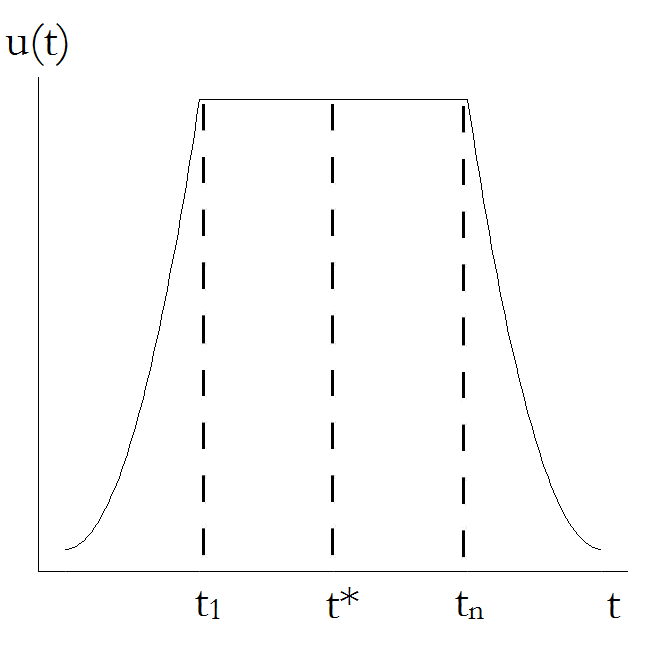
\includegraphics[scale=0.5]{ut.png}
\end{center}

\begin{itemize}
\item
  Since \(u(t)\) is the same \(\forall \ i \in N\), it must be that in
  Nash equilibrium, \(u(t_1)=u(t_2)=...=u(t_n)\). For simplicity assume
  that \(t_1<t_2<...<t_n\) so that each commuter leaves in order.
\item
  One solution is that the departure times \(t_1, t_2, ..., t_n\) are
  uniformly distributed along the plateau. Then, as before,
  \(t_1 = t^* - n/2s \ \wedge \ t_n = t^* + n/2s\). Visually, the
  portion of the utility curve that is at a plateau is of width \(n/s\),
  or the length of the rush hour. We can verify this by observing that
  \(t_n - t_1 = n/s\). This is the same result as when we gave explicit
  utility forms.
\item
  Without an explicit utility form we may still keep some of the same
  notation as before. For example, the length of the queue at time \(t\)
  may still be written as \(D(t)\). We can again define the rate of
  growth for the queue as \(\dot{D}(t) = r(t) - s\). But without an
  explicit utility form we no longer solve for \(r(t)\). In the original
  model we were able to solve that
  \(r(t) = \frac{s \alpha}{\alpha - \beta}\), which implied that the
  queue growed at a constant rate \(r>s\) as long as the commuters
  arrived to work before \(t^*\). In this model we might therefore relax
  the result that the queue grows at a constant rate. For example, on
  the single-plateaued utility function, the solutions
  \(t \in \{t_1,t_2,...,t_n\}\) need not be distributed uniformly, which
  means congestion could grow at different rates determined by \(r(t)\).
\item
  We may also still define \(\tilde{t}\) as the departure time that
  allows the worker to arrive to work at \(t^*\). This again implies
  that \(\tilde{t}+\frac{D(\tilde{t})}{s}=t^*\). \(D(\tilde{t})\) is the
  maximum length that the queue takes. One important result from the
  original model was that \(D(\tilde{t})\), in the original model, did
  not depend on the capacity of the bridge. Here, without a utility
  form, we do not solve for \(D(\tilde{t})\), so we lose that result.
\end{itemize}

\subsubsection{\texorpdfstring{8.7 What happens in the above
generalization if
\(u'(t) < -s\alpha\)?}{8.7 What happens in the above generalization if u'(t) \textless{} -s\textbackslash{}alpha?}}\label{what-happens-in-the-above-generalization-if-ut--salpha}

\begin{itemize}
\tightlist
\item
  In the above generalization, note that for the relevant \(t\),
  \(t \in \{t_1,t_2,...,t_n\}\), we have that \(u'(t) = 0\) on the
  plateau of the utility function. This gives \(u'(t)=0>-\alpha s\).
  Recall that \(\alpha s\) is comprised of \(\alpha\), the cost per
  minute of waiting in traffic, while \(s\) is the number of people let
  through the bottleneck per minute. We need that the marginal utility
  with respect to time is greater than the total cost per minute
  \(\alpha s\) in the system. If the marginal utility is not greater
  than the cost of waiting, \(u'(t)< - \alpha s\), no one should go to
  work.
\end{itemize}

\subsubsection{8.8 Generalize the model to allow two types of commuters
with different preferred times of
arrival.}\label{generalize-the-model-to-allow-two-types-of-commuters-with-different-preferred-times-of-arrival.}

\begin{itemize}
\tightlist
\item
  Let type \(x\) be those who prefer an early arrival time, and type
  \(y\) be those who prefer a later arrival time. Let
  \(t_y^* = t_x^* + \tau\) where \(\tau > 0\). Let \(N = N_x + N_y\).
  Let the traffic wait time cost \(\alpha\) be identical for all people,
  and office arrival penalty \(\beta\) be identical for all people and
  identical for early and late arrivals.
\item
  First note two degenerate cases; the first is when \(\tau = 0\) which
  devolves to the basic case, and the second is when \(\tau\) is very
  large, such that congestion from the two subpopulations do not
  overlap. These cases are both boring, so ignore them.
\item
  Assume that despite the different types, the equilibrium situation
  will result in all commuters having an equal average (dis)utility of
  commuting.
\item
  Note that the very first commuter, leaving at time \(t_1\), must be a
  type \(x\) (a type \(y\) would suffer a greater penalty for arriving
  that much earlier), and the last commuter, leaving at time \(t_N\),
  must be a type \(y\) (a type \(x\) would similarly suffer a greater
  penalty for arriving that much later).
\item
  Note that as long as there is a queue \(D(t) > 0\) in the bottleneck
  at all times between \(t_1\) and \(t_N\), the total traffic jam will
  last \(N/s\) as in the basic problem. Commuter type is irrelevant in
  the flow rate through the bottleneck.

  \begin{align*}
    t_N - t_1 &= \frac{N}{s}\\
    C_1 &= \beta (t_x^* - t_1) 
    &\text{(cost; first commuter is $x$)}\\
    C_N &= \beta (t_N - t_y^*) 
    &\text{(cost; last commuter is $y$)}\\
    C_1 = C_N &\Rightarrow \beta (t_x^* - t_1) = \beta (t_N - t_y^*)
    &\text{(equal costs)}\\
    \Rightarrow \beta (t_x^* - t_1) &= \beta (t_1 + \frac{N}{s} - (t_x^* + \tau))
    &\text{(sub for $t_y^*$ and $t_N$)}\\
    \Rightarrow t_x^* - t_1 &= \frac{N/s - \tau}{2}\\
    \Rightarrow t_N - t_y^* &= \frac{N/s - \tau}{2}
  \end{align*}
\end{itemize}

\begin{center}\rule{0.5\linewidth}{\linethickness}\end{center}

\subsection{Exercises Lecture 9}\label{exercises-lecture-9}

\subsubsection{9.1 A city has 2 types of people, and 1000 people of each
type. There is one private good and one public
good.}\label{a-city-has-2-types-of-people-and-1000-people-of-each-type.-there-is-one-private-good-and-one-public-good.}

Let \(X_i\) denote the amount of private consumption consumed by citizen
\(i\) and let \(Y\) denote the amount of public good available in the
city. All type 1s have the utility function \(U(X_i, Y) = X_iY\), type
2's have the utility function \(U(X_i, Y) = X_iY^2\). The price of
private goods is \$1 per unit. Type 1s have an income of \$10,000 and
Type 2s have an income of \$15,000. Public goods can be made from
private goods with constant returns to scale. It takes 30 units of the
private good to make one unit of the public good. The following
questions relate to alternative arrangements for provision of public
goods in this city.

\begin{enumerate}
\def\labelenumi{\alph{enumi})}
\tightlist
\item
  Calculate the Lindahl equilibrium prices and quantities for this city.
\end{enumerate}

\begin{itemize}
\tightlist
\item
  Type 1
\end{itemize}

\begin{align*}
        & \max \limits_{X_i, Y} X_iY \hspace{10pt} \text{s.t.} \hspace{10pt} 10,000 \geq p_1Y + X_i \\
\end{align*}

FOCs:

\begin{align*}
    &\frac{\dd L}{\dd X_i} = Y - \lambda = 0  \\
    &\frac{\dd L}{\dd Y} = X_i - p_1\lambda = 0  \\
    \Rightarrow & p_1Y = X_i \\
    &\frac{\dd L}{\dd \lambda} = 10,000  =  p_1Y + X_i \\
    \Rightarrow & 10,000 = p_1Y + p_1Y \\
    &\frac{5000}{Y} = p_1
\end{align*}

\begin{itemize}
\tightlist
\item
  Type 2
\end{itemize}

\begin{align*}
        & \max \limits_{X_i, Y} X_iY^2 \hspace{10pt} \text{s.t.} \hspace{10pt} 15,000 \geq p_2Y + X_i \\
\end{align*}

FOCs:

\begin{align*}
    &\frac{\dd L}{\dd X_i} = Y^2 - \lambda = 0  \\
    &\frac{\dd L}{\dd Y} = 2X_iY - p_2\lambda = 0  \\
    \Rightarrow & \frac{p_2Y}{2} = X_i \\
    &\frac{\dd L}{\dd \lambda} = 15,000  =  p_2Y + X_i \\
    \Rightarrow & 15,000 = p_2Y + \frac{p_2Y}{2} \\
    &\frac{10,000}{Y} = p_2 \\
\end{align*}

\begin{itemize}
\tightlist
\item
  Finding the \(Y^*\), \(p_1^*\) and \(p_2^*\)
\end{itemize}

\begin{align*}
    & \sum_{i \in \text{Type 1}} p_1 + \sum_{i \in \text{Type 2}} p_2 = 30 \\
    & 1000*\frac{10,000}{Y} + 1000*\frac{10,000}{Y} = 30 \\
    & \boxed{Y^*=500,000} \\
    \Rightarrow & \hspace{10pt} \boxed{p_1^*=0.01}  \hspace{10pt} \text{and} \hspace{10pt} \boxed{p_2^*=0.02} 
\end{align*}

\begin{enumerate}
\def\labelenumi{\alph{enumi})}
\setcounter{enumi}{1}
\tightlist
\item
  Suppose that the public good is excludable and marketed competitively
  as in the Oakland (1974) model. In the Oakland competitive equilibrium
  with free entry for firms, how many units will be consumed by the type
  1s? the type 2s? What will be the total number of units produced? What
  will the competitive prices be? How many units of the public good will
  the low price seller sell? How much will the high price seller sell.
\end{enumerate}

\begin{itemize}
\tightlist
\item
  From \((a)\) we know that the individual demands for Type 1 and Type 2
  are respectively:
\end{itemize}

\[\frac{5,000}{p} = Y \hspace{10pt} \text{and} \hspace{10pt} \frac{10,000}{p} = Y\]

\begin{itemize}
\item
  The first firm charges such that it covers its cost of provision, i.e.
  \(p_L=\frac{30}{2000}=0.015\). At this price Type 1 folks will demand
  \(\frac{1,000,000}{3}\) and Type 2 \(\frac{2,000,000}{3}\), hence firm
  1 just offers \(\frac{1,000,000}{3}\) to cover its cost.
\item
  Firm 2 now attempts to enter the market and cater to Type 2 folks by
  charging \(p_H=\frac{30}{1000}=0.03\). At this price, Type 2 demand
  the same amount provided under firm 1, hence firm 2 will sell 0
  additional units.
\end{itemize}


\end{document}
